\def\CTeXPreproc{Created by ctex v0.2.9, don't edit!}
%\documentclass{beamer}
\documentclass[%handout,
xcolor=pdftex]{beamer}
\mode<presentation> {
  \usetheme{Warsaw}
  \setbeamercovered{transparent}
}
\let\Tiny=\tiny
\usetheme{Singapore}
\usecolortheme{dolphin}
\usepackage{amsmath}
\usepackage{textcomp}
\usepackage{amssymb}
\usepackage{amsthm}
\usepackage{graphicx}
\usepackage{color}
\usepackage{lipsum}
\usepackage{hyperref}
\usepackage{multirow}
\usepackage{bm}
%\setbeamertemplate{headline}{}
\setbeamertemplate{footline}[page number]
\newcommand\Fontvi{\fontsize{9pt}{8}\selectfont}
\newcommand\Fontvii{\fontsize{7pt}{8}\selectfont}
\newcommand{\backupbegin}{
   \newcounter{finalframe}
   \setcounter{finalframe}{\value{framenumber}}
}
\newcommand{\backupend}{
   \setcounter{framenumber}{\value{finalframe}}
}\newtheorem{proposition}{Proposition}
\title{Unit 5: Exploratory Data Analysis I}
\author[STAT 5170: Applied Time Series, Unit 5]{Taylor R. Brown PhD}
\institute{Department of Statistics, University of Virginia}
\date{Spring 2020}

\AtBeginSubsection[] {
  \begin{frame}<beamer>{Outline}
    \tableofcontents[currentsection,currentsubsection]
  \end{frame}
}

\begin{document}


\frame{\titlepage}


\begin{frame}
\frametitle{Readings for Unit 5}

Textbook chapter 2.2 (pages 54 to 62).

\end{frame}


\begin{frame}
\frametitle{Last Unit}
\begin{enumerate}
\item Linear Regression Overview
\end{enumerate}
\end{frame}

\begin{frame}
\frametitle{This Unit}
\begin{enumerate}
\item Detrending with Linear Regression
\item Differencing for Stationarity
\item Backshift Operator
\end{enumerate}
\end{frame}

\begin{frame}
\frametitle{Motivation}

With time series data, we need to account for the dependence between the values in the series. Stationarity for a time series enables us to measure the dependence, since the dependence structure is regular and does not change over time. When we do not have stationarity, we need methods to reduce the effects of nonstationarity so that stationary properties can be obtained.

\end{frame}

\section{Detrending with Linear Regression}
\frame{\tableofcontents[currentsection]}

\begin{frame}
\frametitle{Detrending with Linear Regression}

Recall that in time series analysis, we prefer to work with stationary processes, to better estimate autocorrelation and other quantities of interest. If our process has a linear trend, we could use linear regression to remove the trend (\textbf{``detrend"}).

\end{frame}

\begin{frame}
\frametitle{Detrending with Linear Regression}

Consider the following model:

\begin{equation} \label{eq:model}
x_t = \mu_t + y_t
\end{equation}

where $y_t$ is a \textbf{zero mean stationary process}, e.g. MA(2), AR(1), white noise, etc., and $\mu_t$ is a \textbf{deterministic trend}, e.g. $\mu_t = \beta_0 + \beta_1 t$.\\
\vspace{5mm}
We can view $x_t$ as having stationary behavior around a trend. A strong trend, $\mu_t$, can obscure the behavior of the stationary process, $y_t$. Hence, we may want to remove the trend as a first step in exploratory analysis of such time series, especially if the goal is to understand the behavior of $y_t$.

\end{frame}

\begin{frame}
\frametitle{Detrending with Linear Regression}

The steps involved are

\begin{itemize}
\item Obtain an \textbf{estimate} of the trend component, $\hat{\mu_t}$, e.g. via OLS.
\item Work with the residuals $e_t = x_t - \hat{\mu_t}$.
\end{itemize}

\end{frame}

\begin{frame}
\frametitle{Back to Marriages in Church of England}

Recall in this earlier example that a regression of marriages in the Church of England against time should include a quadratic term, so the trend is

$$
\mu_t = \beta_1 + \beta_2 t + \beta_3 t^2.
$$

Using OLS regression, we obtained

$$
\hat{\mu_t} = -15130 + 16.43 t - 0.00444 t^2.
$$

\end{frame}

\begin{frame}
\frametitle{Back to Marriages in Church of England}

The detrended series is obtained by subtracting $\hat{\mu_t}$ from the observed values $x_t$

$$
e_t = x_t + 15130 - 16.43 t + 0.00444 t^2.
$$

Next, we observe the plot of $e_t$ and its ACF.

\end{frame}

\begin{frame}
\frametitle{Back to Marriages in Church of England}

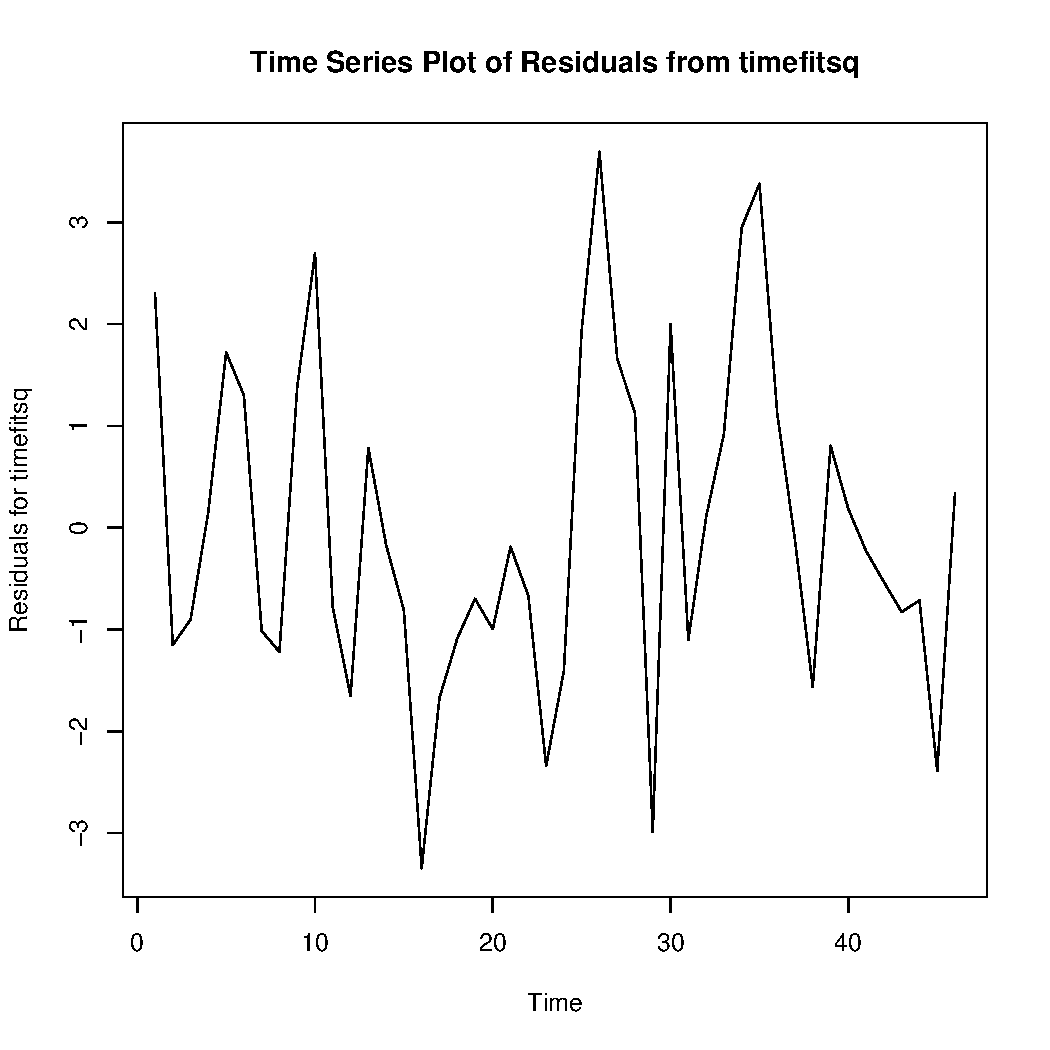
\includegraphics[width=100mm, height=60mm]{pics/restimefitsq.pdf}

\end{frame}

\begin{frame}
\frametitle{Back to Marriages in Church of England}

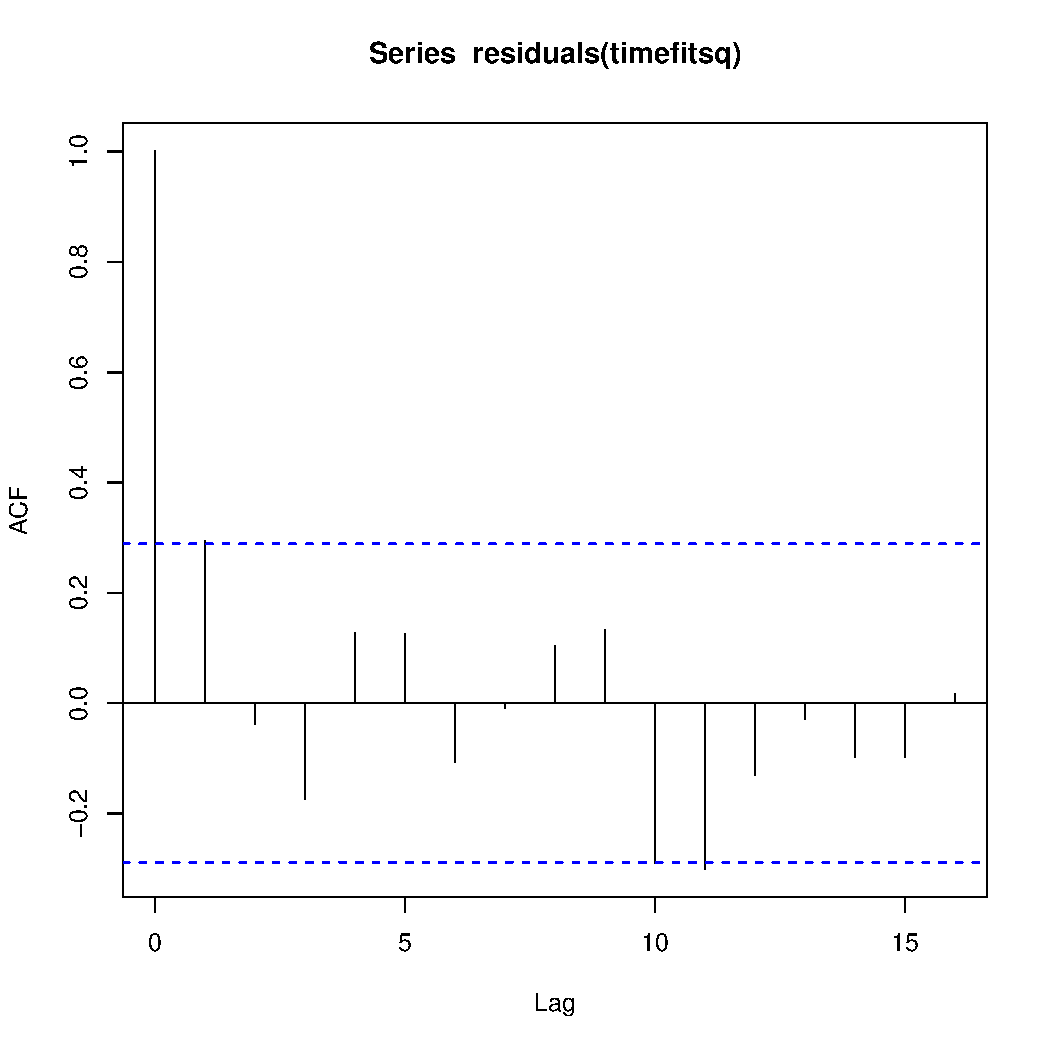
\includegraphics[width=100mm, height=60mm]{pics/acftimefitsq.pdf}

\end{frame}

\begin{frame}
\frametitle{Summary of Detrending}

We find a good point estimate of $\mu_t$ and then look at the residuals
$$
e_t=x_t-\hat{\mu}_t.
$$

One thing we could do is to ``detrend'' with linear regression, e.g. use OLS regression to obtain $\hat{\mu_t} = \hat{\beta_1} + \hat{\beta_2} t$. With the residuals, based on the structure of their ACF, we have an idea on the model that may reasonably describe the stationary process $y_t$.

\end{frame}

\begin{frame}
\frametitle{Summary of Detrending}

\textbf{Question:} What is an implication if the residuals after detrending have a pattern / trend?

\vspace{50mm}

\end{frame}



\section{Differencing for Stationarity}
\frame{\tableofcontents[currentsection]}




\begin{frame}
\frametitle{Differencing}

Let $\nabla$ denote the differerncing operation. Applying $\nabla$ to $x_t$ results in

\begin{equation} \label{eq:first}
\nabla x_t = x_t-x_{t-1},
\end{equation}

which is also called the \textbf{first difference}.


\end{frame}

\begin{frame}
\frametitle{Differencing}

Suppose we assume the trend component $\mu_t$ follows a simple linear regression, then

\begin{eqnarray*}
\nabla x_t &=& \nabla (\beta_0 + \beta_1 t + y_t) \\
           &=&  \\
           &=&
\end{eqnarray*}

Notice that the detrending may give us a more accurate representation of $y_t$, whereas differencing completely \textbf{removes} $\beta_0$ and turns $\beta_1$ into the \textbf{mean} of the series $\{\nabla x_t \}$.

\end{frame}

\begin{frame}
\frametitle{Differencing}

However, differencing changes $y_t$ and often introduces
additional dependency. Consider regression with MA(1).
$$
x_t=\beta_0+\beta_1 t +w_t+\theta_1 w_{t-1}
$$
Differencing the above expression, we have
\begin{eqnarray*}
\nabla x_t &=& \nabla (\beta_0)  + \nabla(\beta_1 t) + \nabla w_t + \theta_1 \nabla w_{t-1} \\
           &=& \\
           &=&
\end{eqnarray*}

which becomes a mean value $\beta_1$ plus MA(2). $\{\nabla x_t \}$ is stationary.

\end{frame}

\begin{frame}
\frametitle{Differencing}

\textbf{Question:} Suppose instead of a trend, $\mu_t$ follows a random walk with drift process, derive $\nabla x_t$.

\vspace{50mm}

\end{frame}

\begin{frame}
\frametitle{Differencing Vs Detrending}

\begin{itemize}
\item An advantage of differencing over detrending is that no parameters are estimated in the differencing operation.
\item A disadvantage of differencing is that it does not provide an estimate of the stationary process $y_t$.
\end{itemize}

\end{frame}

\begin{frame}
\frametitle{Differencing Vs Detrending}

\begin{itemize}
\item If estimating $y_t$ is the goal, then \textbf{detrending} may be more appropriate.
\item If the goal is to make the data stationary, then \textbf{differencing} may be more appropriate.
\end{itemize}

\end{frame}

\section{Backshift Operator}
\frame{\tableofcontents[currentsection]}

\begin{frame}
\frametitle{Backshift Operator}

The \textbf{backshift operator} is defined as

\begin{equation*}
B x_t = x_{t-1},
\end{equation*}

which can be extended to powers

\begin{equation}
B^k x_t = x_{t-k}.
\end{equation}

\end{frame}

\begin{frame}
\frametitle{Backshift Operator}

Thus, the first difference (\ref{eq:first}) can be written as

\vspace{50mm}

\end{frame}

\begin{frame}
\frametitle{Backshift Operator}

\textbf{Question:} Denote the second difference, $\nabla^2 x_t$ in terms of the backshift operator.

\vspace{50mm}

\end{frame}

\begin{frame}
\frametitle{Backshift Operator}

In general, for all positive integer $d$,
\begin{equation}
\nabla^d = (1-B)^d.
\end{equation}

\end{frame}

\begin{frame}
\frametitle{Backshift Operator}

We showed earlier that the first difference eliminates a linear trend. This is an example of a \textbf{linear filter} applied to eliminate a linear trend. Next, we show that the second difference eliminates a quadratic trend.

\vspace{50mm}

\end{frame}

\section{Worked Example}
\frame{\tableofcontents[currentsection]}

\begin{frame}
\frametitle{Example: Global Temperature}

Let's look at average global temperatures from 1900 to 1997. The data are measured in deviation in degrees centigrade from the 1961-1990 average.

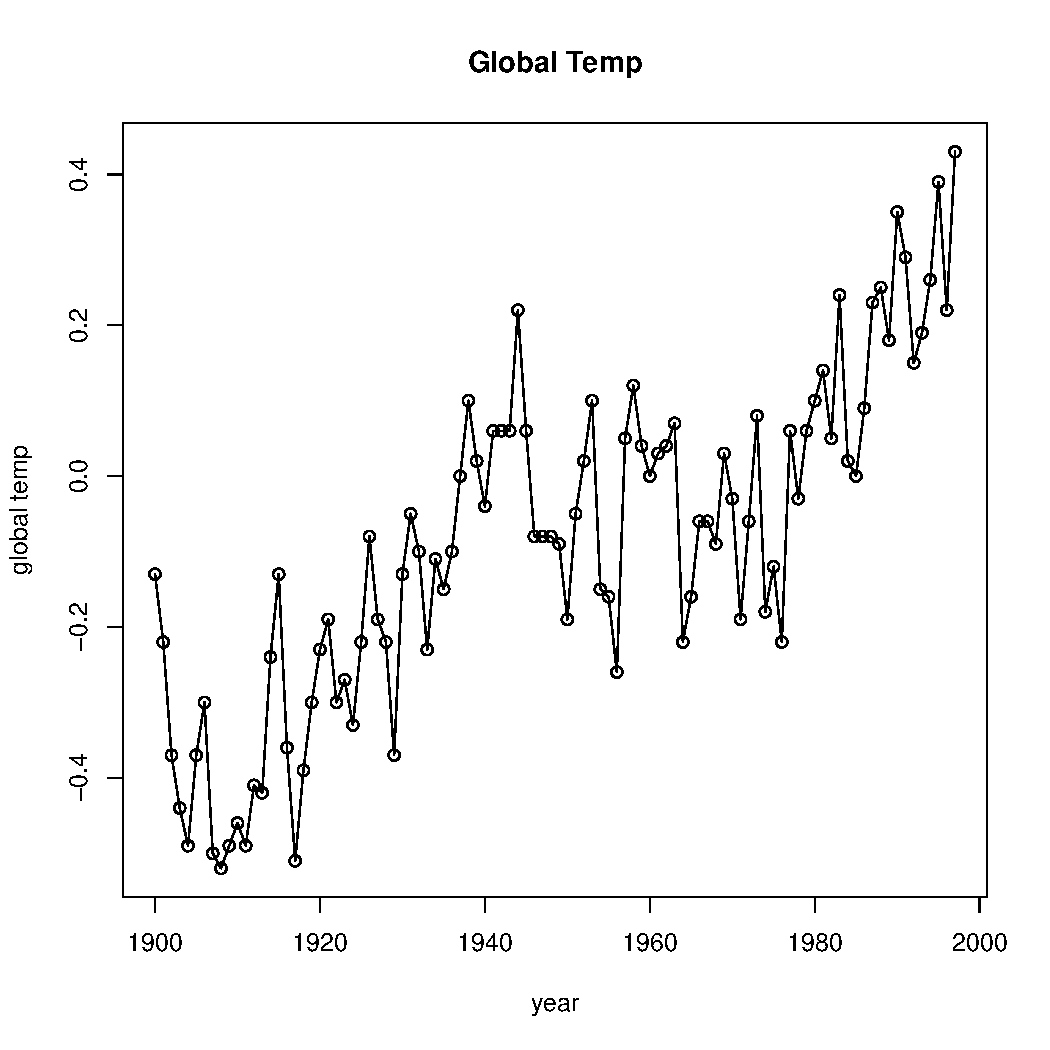
\includegraphics[width=100mm, height=60mm]{pics/plots1.pdf}

\end{frame}

\begin{frame}
\frametitle{Example: Global Temperature}

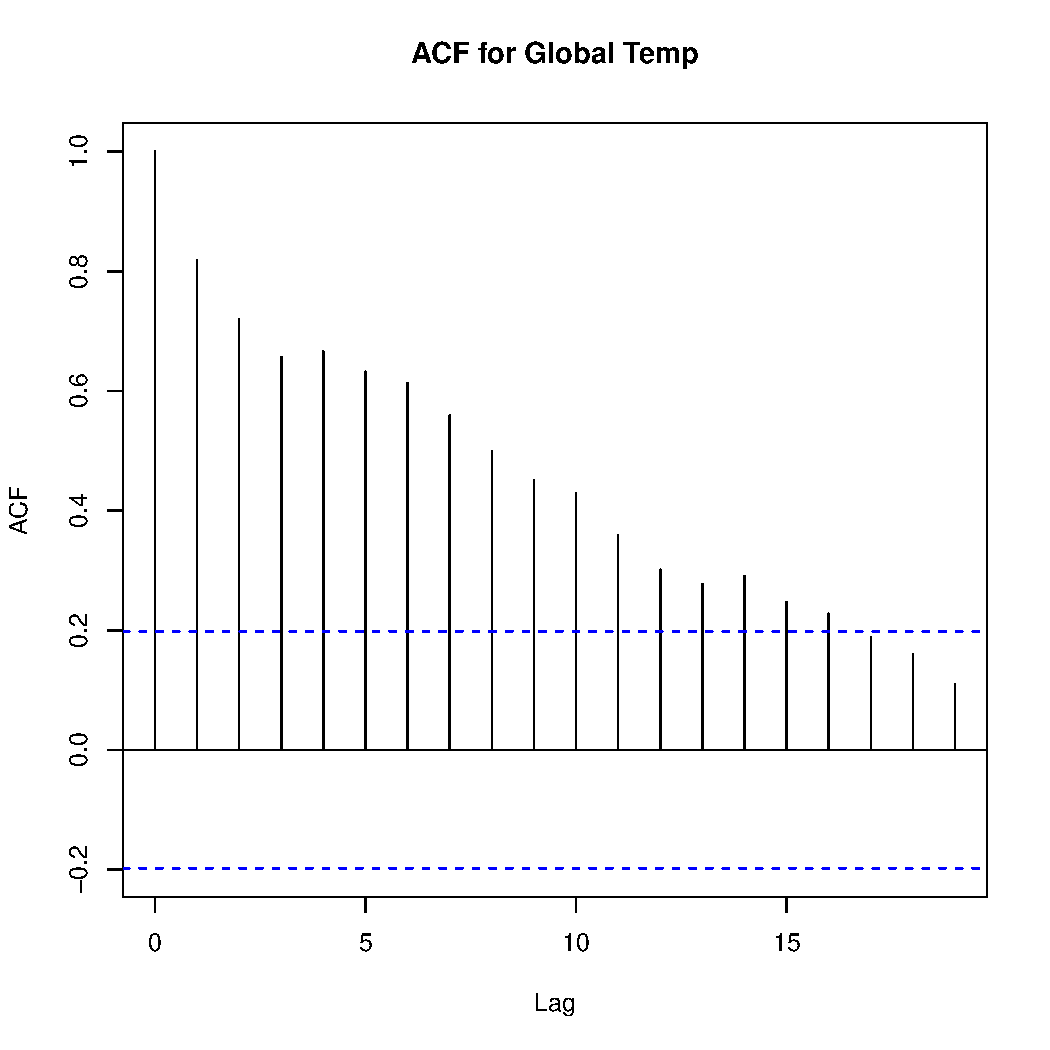
\includegraphics[width=100mm, height=60mm]{pics/acf1.pdf}

\textbf{Question}: What does this indicate about stationarity?

\end{frame}

\begin{frame}
\frametitle{Example: Global Temperature}

Next, we look at detrended data.

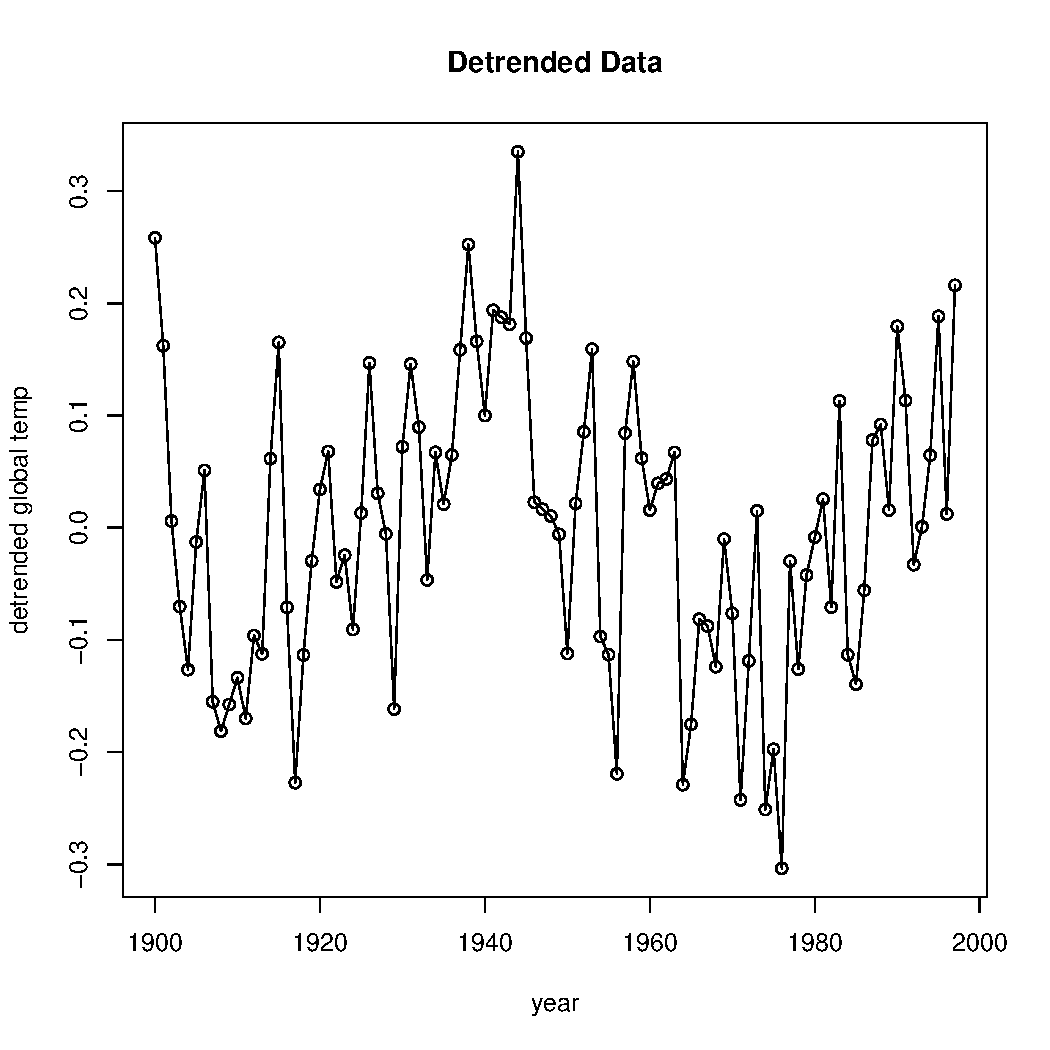
\includegraphics[width=100mm, height=60mm]{pics/plots2.pdf}

\end{frame}

\begin{frame}
\frametitle{Example: Global Temperature}

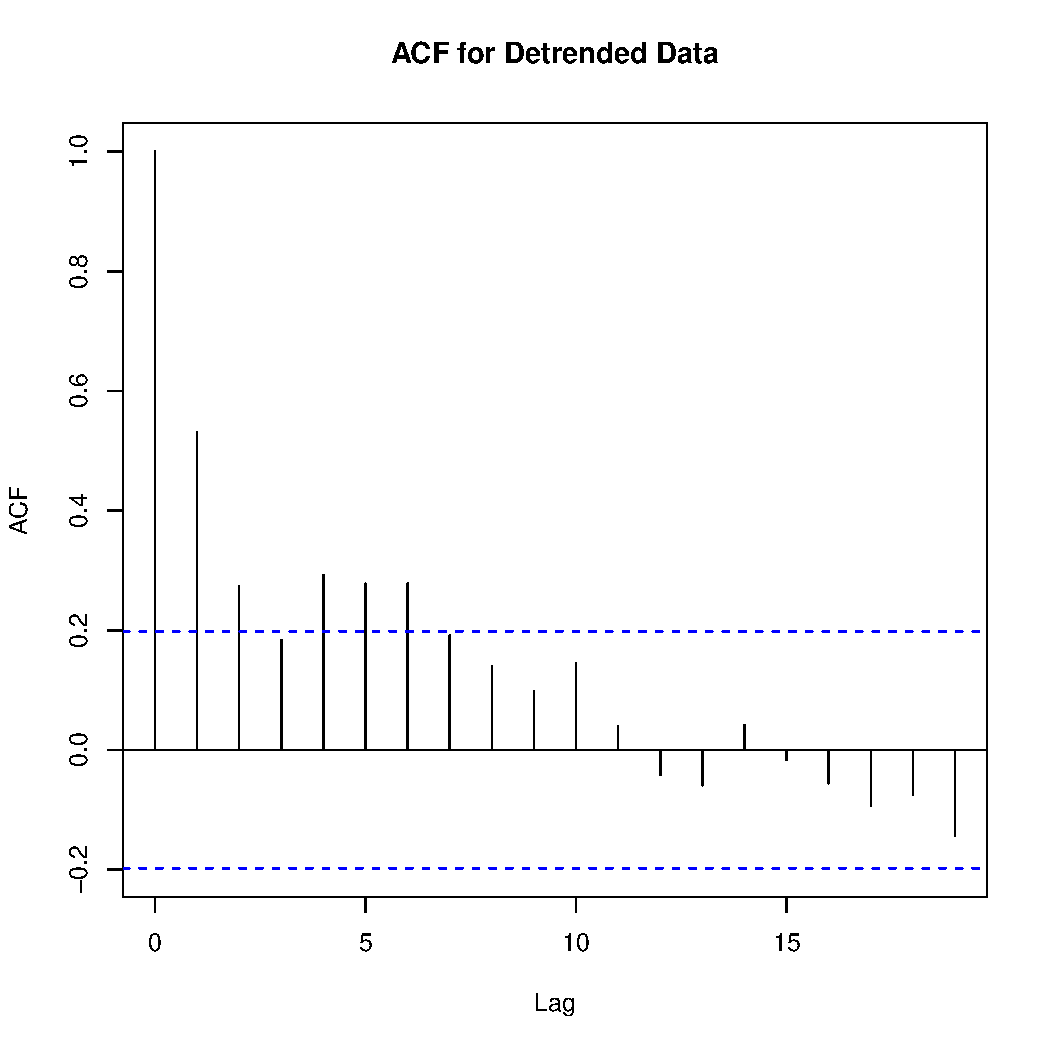
\includegraphics[width=100mm, height=60mm]{pics/acf2.pdf}

\end{frame}

\begin{frame}
\frametitle{Example: Global Temperature}

Finally, we look at differenced data.

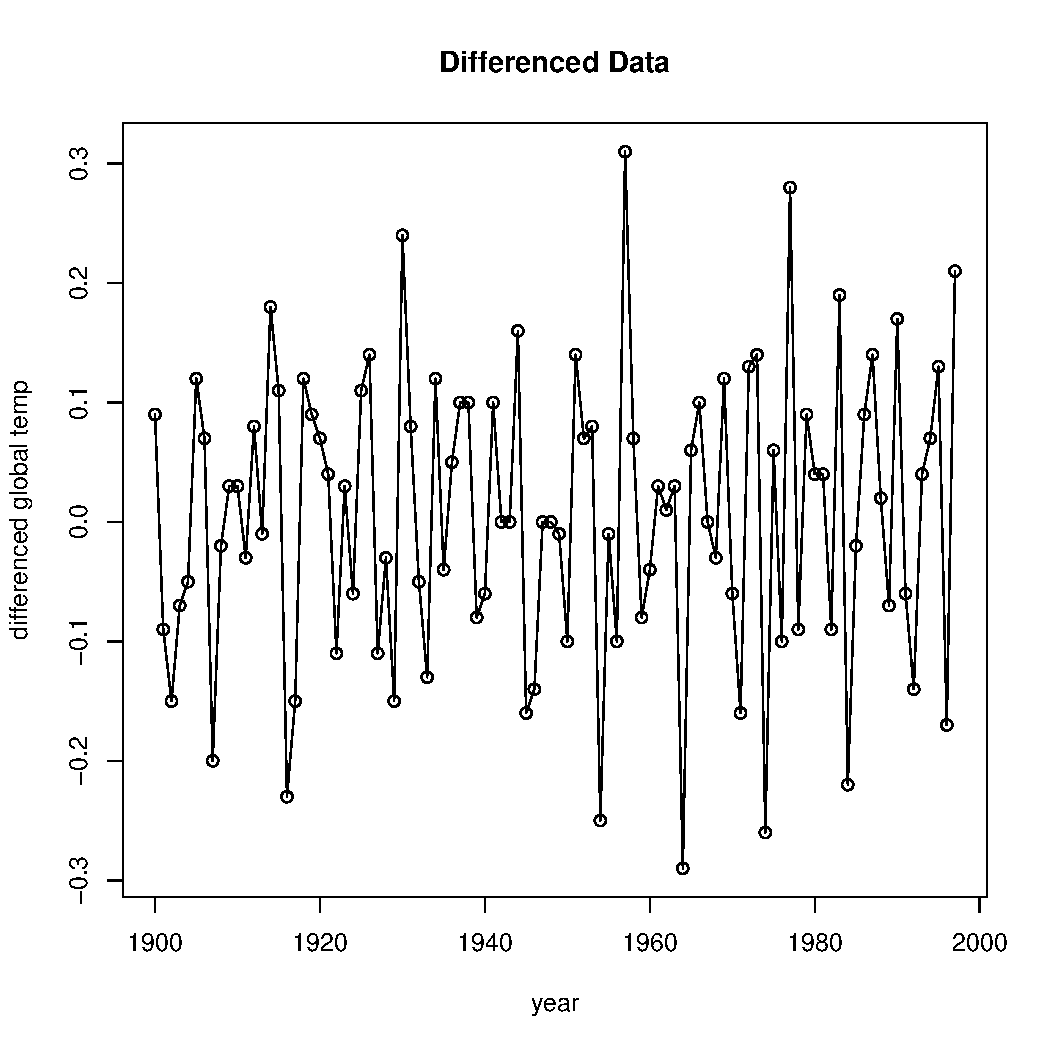
\includegraphics[width=100mm, height=60mm]{pics/plots3.pdf}

\end{frame}



\begin{frame}
\frametitle{Example: Global Temperature}

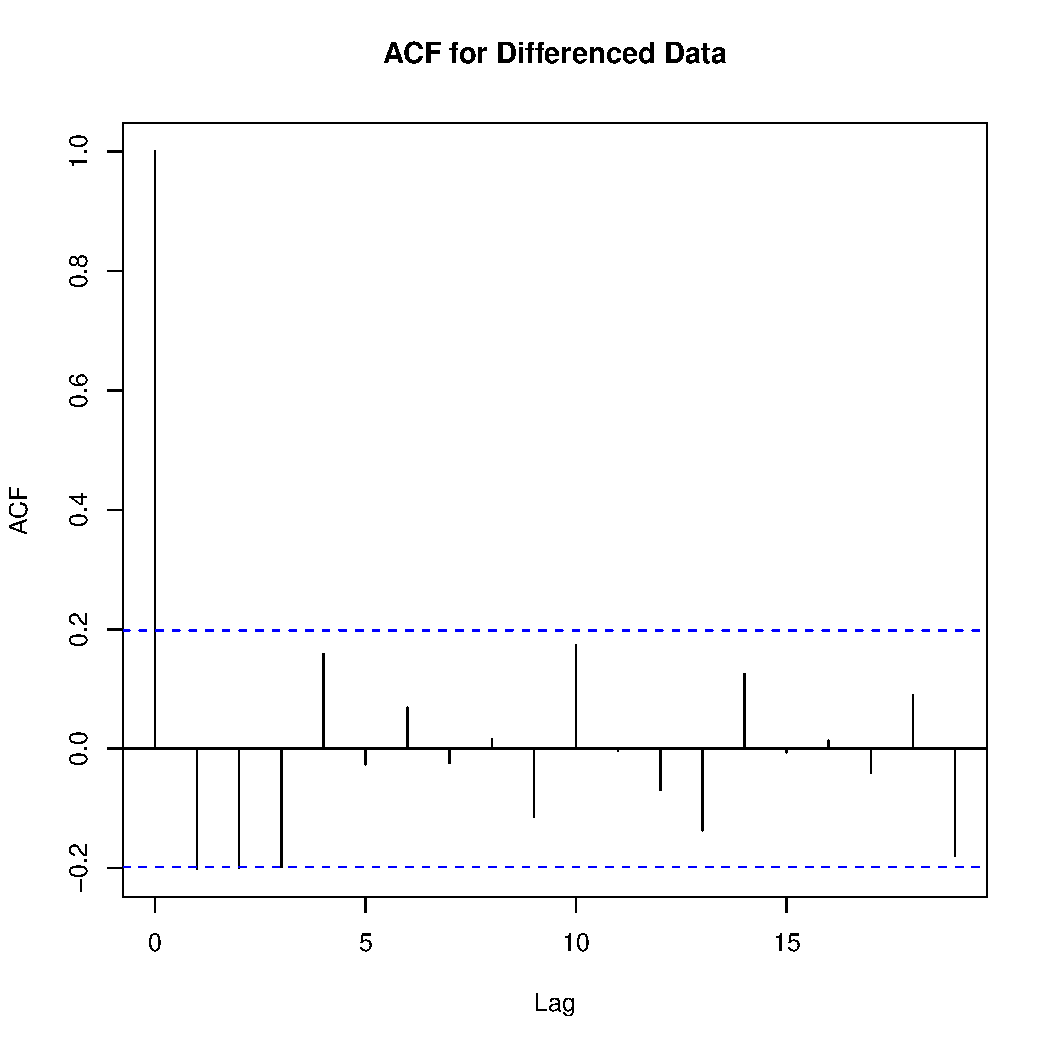
\includegraphics[width=100mm, height=60mm]{pics/acf3.pdf}

\end{frame}

\begin{frame}
\frametitle{Example: Global Temperature}

\textbf{Question:} Based on the plots and ACFs, what can we say about the behavior of global temperature?

\vspace{50mm}

\end{frame}

\begin{frame}
\frametitle{Example: Global Temperature}

\textbf{Question:} How would you estimate the parameters of the process you are considering for the behavior of global temperature?

\vspace{50mm}

\end{frame}




\end{document} 